\clearpage

\section{Theoretical Analysis}
\label{sec:analysis}

In this part we will discuss the theoretical analysis of the circuit shown in figure \ref{fig:Principal}.
The values used for $R_1$, $C_1$, $R_2$, $C_2$, $R_3$ and $R_4$ are the same as the ones used in \textit{Ngspice}, so it is easier
to compare both analyses. Even though we could do the calculations with the actual model presented in figure
\ref{fig:Principal}, we decided to use the incremental model presented in figure \ref{fig:Incremental}, below, since it makes calculations easier.

\begin{figure}[h] \centering
    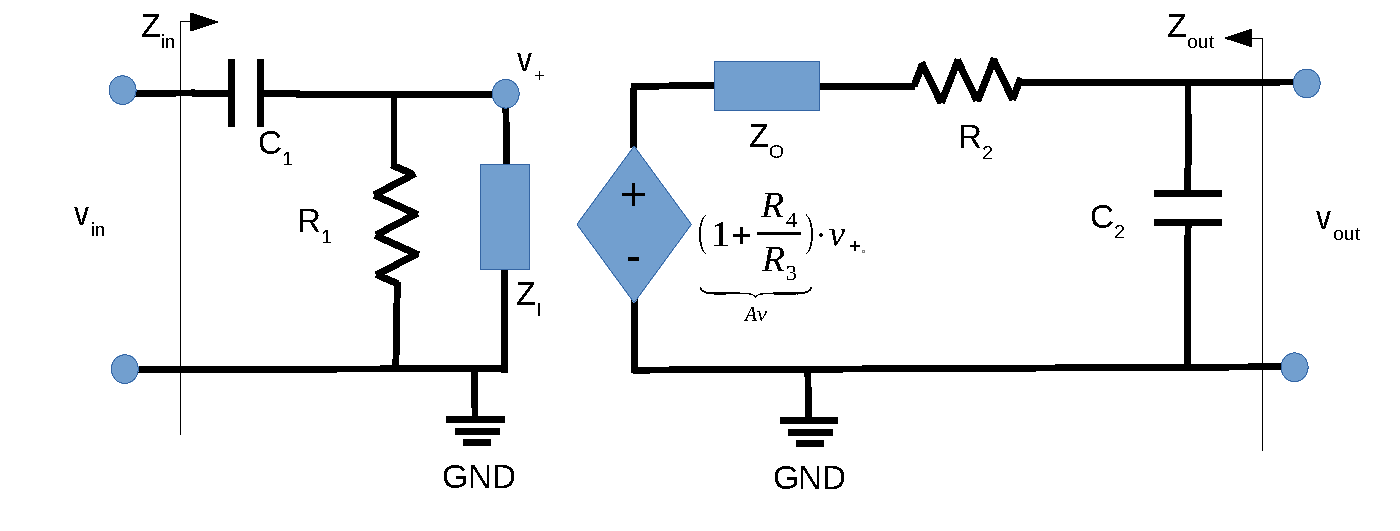
\includegraphics[scale=0.65]{lab5_incremental.pdf}
    \caption{Band-pass filter incremental circuit.}
    \label{fig:Incremental}
\end{figure}

The gain associated with the dependent voltage source is given by $1+\frac{R_4}{R_3}$, since the amplifier subcircuit 
corresponds to a non-inverting amplifier. 

The OP-AMP is considered to be ideal, so $Z_I=\infty$ (behaves like an open circuit) and $Z_O=0$ (behaves like a short circuit).
Additionally, it is know that $v_{+}=v_{-}$ (would be needed if we did not use the incremental model).
This way, we can determine the expression for the gain using only the two voltage divider relations below:

\begin{equation}\label{eq:2}
  v_{+}=\frac{R_1}{R_1+Z_{C_1}}v_{in}
\end{equation}

\begin{equation}
  v_{out}=\frac{Z_{C_2}}{Z_{C_2}+R_2}v_{+}A_v=(\frac{Z_{C_2}}{Z_{C_2}+R_2})(\frac{R_1}{R_1+Z_{C_1}})(1+\frac{R_4}{R_3})v_{in}
\end{equation} 

where $Z_{C_1}=\frac{1}{j \omega C_1}$ and $Z_{C_2}=\frac{1}{j \omega C_2}$. This way the gain is given by equation \ref{eq:gain}:

\begin{equation}
  \frac{v_{out}}{v_{in}}=(\frac{Z_{C_2}}{Z_{C_2}+R_2})(\frac{R_1}{R_1+Z_{C_1}})(1+\frac{R_4}{R_3})
  \label{eq:gain}
\end{equation} 

Computing the absolute value of the gain (in dB), for a frequency vector in log scale with 10 points per decade,
from $10$ Hz to $100$ MHz, we obtained the graphic in figure \ref{fig:MatGain_dB}. Computing the phase we obtained the graphic in figure \ref{fig:MatPhase}. 

\clearpage

%%%%% GRAFICO GAIN
\vspace{-0.25cm}
\begin{figure}[h] \centering
  \includegraphics[scale=0.55]{Octave_t5.pdf}
  \caption{\emph{Octave} gain in dB.}
  \label{fig:MatGain_dB}
\end{figure}

%%%%% GRAFICO PHASE
\begin{figure}[h] \centering
    \includegraphics[scale=0.55]{Octave_t5p.pdf}
    \caption{\emph{Octave} gain's phase.}
    \label{fig:MatPhase}
\end{figure}

\clearpage

Since we know that the cut-off frequencies correspond to a gain $3$ dB lower than the maximum gain, we were able to find the lower cut-off frequency, $f_L$, 
and the upper cut-off frequency, $f_H$. The central frequency, $f_c$, 
is then given by the geometric mean of the two cut-off frequencies, given by equation \ref{eq:fc}:

\begin{equation}
  f_c = \sqrt{f_L \times f_H}
\label{eq:fc}
\end{equation}

The values for $f_L$, $f_H$ and $f_c$, as well as the gain at the central frequency, are shown in tables \ref{tab:MatFreqs} and \ref{tab:MatGain}.

\begin{table}[h]
    \parbox{.45\linewidth}{
      \centering
      %%%%%%%%%%%%%%%%%% TABELA FREQUENCIAS
      \begin{tabular}{|c|c|}
        \hline
        {\bf Name} & {\bf Value [Hz]} \\ \hline
        \input{../mat/Freq_tab.tex}
      \end{tabular}
      \caption{\emph{Octave}'s cut-off frequencies and central frequency.}\label{tab:MatFreqs}
    }
    \hfill
    \parbox{.45\linewidth}{
      \centering
      %%%%%%%%%%%%%%%%%% TABELA GAIN AT CENTRAL FREQUENCY 
      \begin{tabular}{|c|c|}
        \hline
        {\bf Name} & {\bf Value [dB or -]} \\ \hline
        \input{../mat/Gain_tab.tex}
      \end{tabular}
      \caption{\emph{Octave}'s gain in dB and linear gain.}\label{tab:MatGain}
    }
\end{table}

Finally, we calculated the input and output impedances of the circuit at the central frequency.

For the input impedance, $Z_{in}$, we considered an output load $Z_L=\infty$, and an input voltage source with the central frequency.
 Since $Z_I=\infty$ and behaves like an open circuit, $Z_{in}$ is simply given by the impedances of $C_1$ and $R_1$ in series, as in equation \ref{eq:ZI}:

\begin{equation}
  Z_{in} = R_1 + Z_{C_1}
\label{eq:ZI}
\end{equation}

For the output impedance, $Z_{out}$, we considered a null input voltage and an output voltage source with the central frequency.
Since there is no input voltage, $v_{+}=0$, as we can confirm using the voltage divider (equation (\ref{eq:2})), and consequently the dependent voltage 
source acts like a short circuit. This way, since $Z_O=0$, $Z_{out}$ is simply given by the impedances of $C_2$ and $R_2$ in parallel,
as in equation \ref{eq:ZO}:   

\begin{equation}
  Z_{out} = \frac{R_2 Z_{C_{2}}}{R_2 + Z_{C_{2}}}
\label{eq:ZO}
\end{equation}

$Z_{in}$ and $Z_{out}$ are computed at the central frequency. The results are shown in table \ref{tab:MatZ}.


%%%%%%%%%%%%%%%% TABELA IMPENDANCES
\begin{table}[h]
    \centering
    \begin{tabular}{|c|c|}
      \hline
      {\bf Name} & {\bf Value [$\Omega$]} \\ \hline
      \input{../mat/Imp_tab.tex}
    \end{tabular}
    \vspace{-2.5mm}
    \caption{\emph{Octave}'s input and output impedances' absolute values.}\label{tab:MatZ}
\end{table}

\clearpage

\section{Comparison}\label{sec:Comparison}

In this section we present \emph{Ngspice}'s and \emph{Octave}'s results side by side, so it is easier to compare the two.

\subsection{Gain plots}
%%%%% GRAFICO GAIN NGSPICE
\begin{figure}[h] \centering
    \includegraphics[scale=0.45]{sim_gain_db.pdf}
    \caption{\emph{Ngspice}'s gain in dB}
    \label{fig:SimGain_Comp}
\end{figure}

%%%%% GRAFICO GAIN OCTAVE
\begin{figure}[h] \centering
    \includegraphics[scale=0.475]{Octave_t5.pdf}
    \caption{\emph{Octave}'s gain in dB.}
    \label{fig:MatGain_dB_Comp}
\end{figure}

\clearpage

\subsection{Phase plots}
%%%%% GRAFICO PHASE NGSPICE
\begin{figure}[h] \centering
    \includegraphics[scale=0.45]{sim_phase.pdf}
    \caption{\emph{Ngspice}'s phase plot.}
    \label{fig:SimPhase_Comp}
\end{figure}

%%%%% GRAFICO PHASE OCTAVE
\begin{figure}[h] \centering
    \includegraphics[scale=0.5]{Octave_t5p.pdf}
    \caption{\emph{Octave}'s phase plot.}
    \label{fig:MatPhase_Comp}
\end{figure}

\clearpage

\subsection{Frequency tables}
\begin{table}[h]
    \parbox{.45\linewidth}{
      \centering
      %%%%%%%%%%%%%%%%%% TABELA FREQUENCIAS NGSPCICE
      \begin{tabular}{|c|c|}
        \hline
        {\bf Name} & {\bf Value [Hz]} \\ \hline
        \input{../sim/SimFreqs_tab.tex}
      \end{tabular}
      \caption{\emph{Ngspice}'s cut-off frequencies and central frequency.}\label{tab:SimFreqs_Comp}
    }
    \hfill
    \parbox{.45\linewidth}{
      \centering
      %%%%%%%%%%%%%%%%%% TABELA FREQUENCIAS OCTAVE
      \begin{tabular}{|c|c|}
        \hline
        {\bf Name} & {\bf Value [Hz]} \\ \hline
        \input{../mat/Freq_tab.tex}
      \end{tabular}
      \caption{\emph{Octave}'s cut-off frequencies and central frequency.}\label{tab:MatFreqs_Comp}
    }
\end{table}


\subsection{Gain tables}
\begin{table}[h]
    \parbox{.45\linewidth}{
      \centering
      %%%%%%%%%%%%%%%%%% TABELA GAIN NGSPCICE
      \begin{tabular}{|c|c|}
        \hline
        {\bf Name} & {\bf Value [dB or -]} \\ \hline
        \input{../sim/SimGain_tab.tex}
      \end{tabular}
      \caption{\emph{Ngspice}'s gain in dB and linear gain.}\label{tab:SimGain_Comp}
    }
    \hfill
    \parbox{.45\linewidth}{
      \centering
      %%%%%%%%%%%%%%%%%% TABELA GAIN OCTAVE
      \begin{tabular}{|c|c|}
        \hline
        {\bf Name} & {\bf Value [dB or -]} \\ \hline
        \input{../mat/Gain_tab.tex}
      \end{tabular}
      \caption{\emph{Octave}'s gain in dB and linear gain.}\label{tab:MatGain_Comp}
    }
\end{table}


\subsection{Input and output impedances (at central frequency) tables}
\begin{table}[h]
    \parbox{.45\linewidth}{
      \centering
      %%%%%%%%%%%%%%%%%% TABELA IMPEDANCES NGSPCICE
      \begin{tabular}{|c|c|}
        \hline
        {\bf Name} & {\bf Value [$\Omega$]} \\ \hline
        \input{../sim/SimZ_tab.tex}
      \end{tabular}
      \caption{\emph{Ngspice}'s input and output impedances' absolute values.}\label{tab:SimZ_Comp}
    }
    \hfill
    \parbox{.45\linewidth}{
      \centering
      %%%%%%%%%%%%%%%%%% TABELA IMPEDANCES OCTAVE
      \begin{tabular}{|c|c|}
        \hline
        {\bf Name} & {\bf Value [$\Omega$]} \\ \hline
        \input{../mat/Imp_tab.tex}
      \end{tabular}
      \caption{\emph{Octave}'s input and output impedances' absolute values.}\label{tab:MatZ_Comp}
    }
\end{table}

As one may notice, there are a few differences when comparing \textit{Ngspice}'s and \textit{Octave}'s results.
This is somewhat normal, since the OP-AMP is composed of several transistors, which are non linear, and the model 
used in the theoretical analysis to describe it is the ideal model, which is far from reality. On the other hand,
the model used in \textit{Ngspice} is far more complex. Despite this, the results are quite satisfactory. 
The most notable difference is in between the two phase plots. This can be explained, once again, by the fact that
we use the ideal OP-AMP model for the theoretical analysis, whereas \emph{Ngspice} uses a real model, which in
turn results in the introduction of two more poles in the transfer function, which end up changing the overall aspect
of the phase plot.